\chapter{Modelação}
De forma a respondermos às necessidades do enunciado proposto, iniciamos por realizar as alterações necessárias à rede de distribuição de electricidade, tendo em conta o número mecanográfico 84610, seguido da formulação do modelo para atingir o objectivo proposto de minimização da distância total percorrida, garantindo que todas as arestas serão percorridas.
\begin{figure}[h!]
\centering
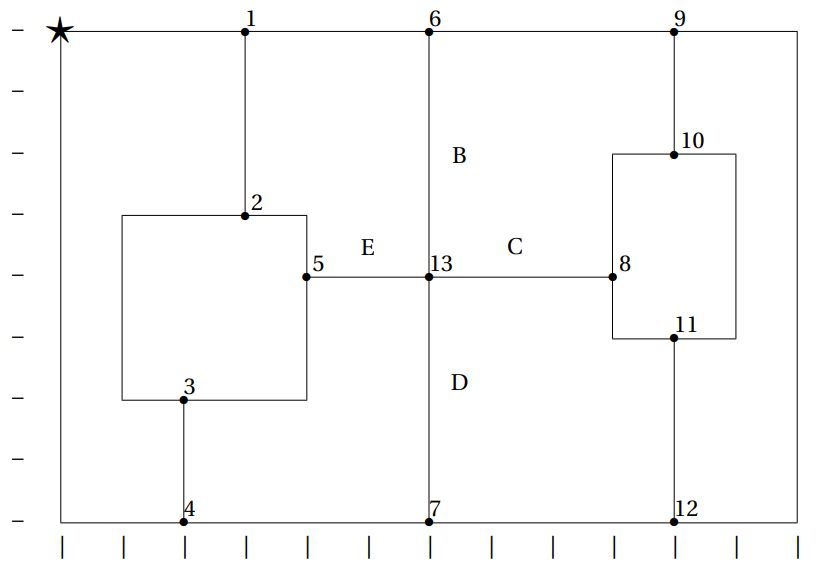
\includegraphics[width=.85\textwidth]{images/main/redeOriginal.png}
\caption{Rede original}
\end{figure}
\newpage
\section{Remoção de Arestas}
Como proposto pelo enunciado, começamos por alterar a rede com as devidas arestas removidas. Teremos então que remover a aresta B, C e D (número 84610).

\begin{figure}[h!]
\centering
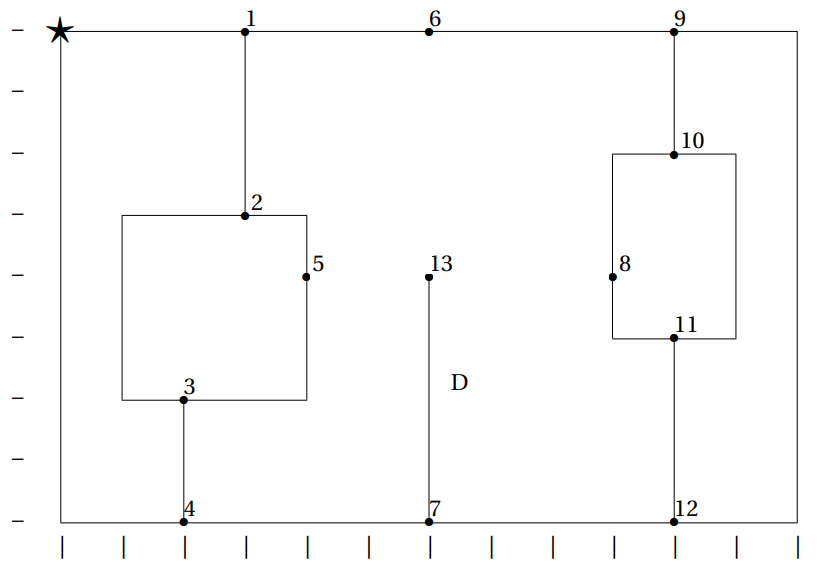
\includegraphics[width=.85\textwidth]{images/main/novaRede.png}
\caption{Nova rede}
\end{figure}

\section{Formulação do Problema}


O problema consiste na minimização do custo, a nível de distância, do percurso do drone de forma a percorrer todas as arestas necessárias pelo menos uma vez. 

As distancias euclidianas estão definidas da seguinte forma:
\begin{figure}[h!]
\centering
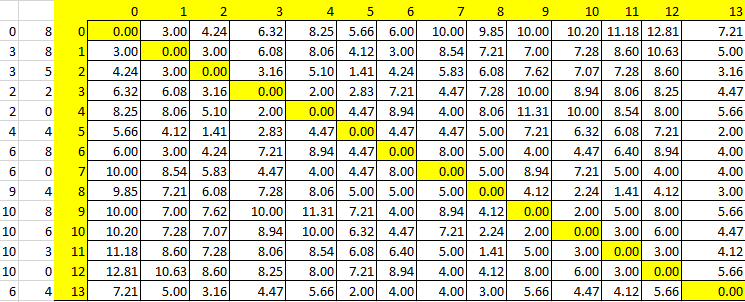
\includegraphics[width=.85\textwidth]{images/main/distancias.png}
\caption{Distâncias Euclidianas}
\end{figure}

Para alcançar o objectivo proposto, optamos por definir as seguintes variáveis de decisão:

$x_{ij} \in \field{N}$: número de vezes que é percorrido o trajecto direto mais curto com origem no vértice $i$ e destino $j$. Para vértices adjacentes, esta variável corresponde frequentemente à aresta entre os mesmos.

$x_{ij}a \in \field{N}$: número de vezes que é percorrida a aresta com origem em $i$ e destino $j$, para os casos em que a aresta entre $i$ e $j$ adjacentes não corresponde ao trajeto mais curto possível entre estes.

\subsection{Função objectivo}



Sendo o nosso objetivo encontrar uma solução ótima para o problema de percorrer todas as arestas, concluímos que se trata de um problema de minimização, onde estamos a tentar encontrar o caminho mais curto possível, ou seja, com a mínima distância total. Para tal, formulamos a seguinte função objetivo:

min: $\sum_{i=0}^{k} n_{i} *x_{i}$

Onde $i$ corresponde a um trajeto específico entre dois vértices, $n_i$ à distância correspondente a esse trajeto, e $x_{i}$ o número de vezes que esse trajeto é percorrido, com $k$ o número total de trajetos disponíveis.

\subsection{Restrições}

De modo a certificar que iremos obter uma solução correta, tivemos também de considerar as restrições a serem usadas no nosso modelo. Para tal, implementamos as seguintes restrições:

\subsubsection{Arestas todas percorridas}
$x_{ij} + x_{ji} >= 1$, para todo $x_{ij}$ correspondente a uma aresta, entre $i$ e $j$. Esta restrição serve para certificar que todas as arestas são percorridas, pelo menos uma vez, independentemente da direção;

\subsubsection{Entrada e Saída de Vértices}

$\sum_{i=0}^{k} x_{ij} = \sum_{i=0}^{k} x_{ji}$, $k\in \field{N}$. Com esta restrição, pretendemos garantir que para cada caminho com destino numa aresta, existe um com origem dessa mesma aresta. Com isto garantimos um caminho aceitável, e que é possível de percorrer.

\section{Modelação em LpSolve (input)}

\subsection{Função objetivo:}
Transferimos a nossa função objetivo para lpsolve, com o objetivo de minimizar o custo total do percurso.
\begin{figure}[h!]
\centering
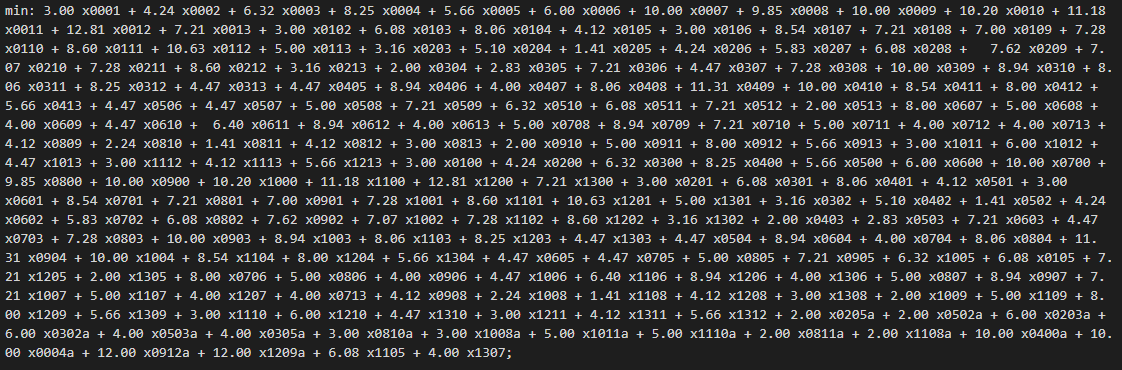
\includegraphics[width=1\textwidth]{images/main/FuncaoObjetivo.png}
\caption{Função objectivo}
\end{figure}


\subsection{Restrições}

\subsubsection{Arestas todas percorridas}
Foram adicionadas ao LpSolve as restrições que certificam que todas as arestas são percorridas, pelo menos uma vez, em qualquer direção.


\begin{figure}[h!]
\centering
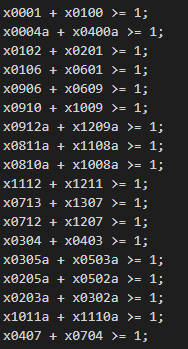
\includegraphics{images/main/restricoesTodasArestas2.png}
\caption{Restrições para as arestas serem todas percorridas}
\end{figure}


\subsubsection{Entrada e Saída de Vértices}
Foram adicionadas também restrições para garantir que o número de entradas num vértice corresponde ao número de saídas do mesmo.

\begin{figure}[h!]
\centering
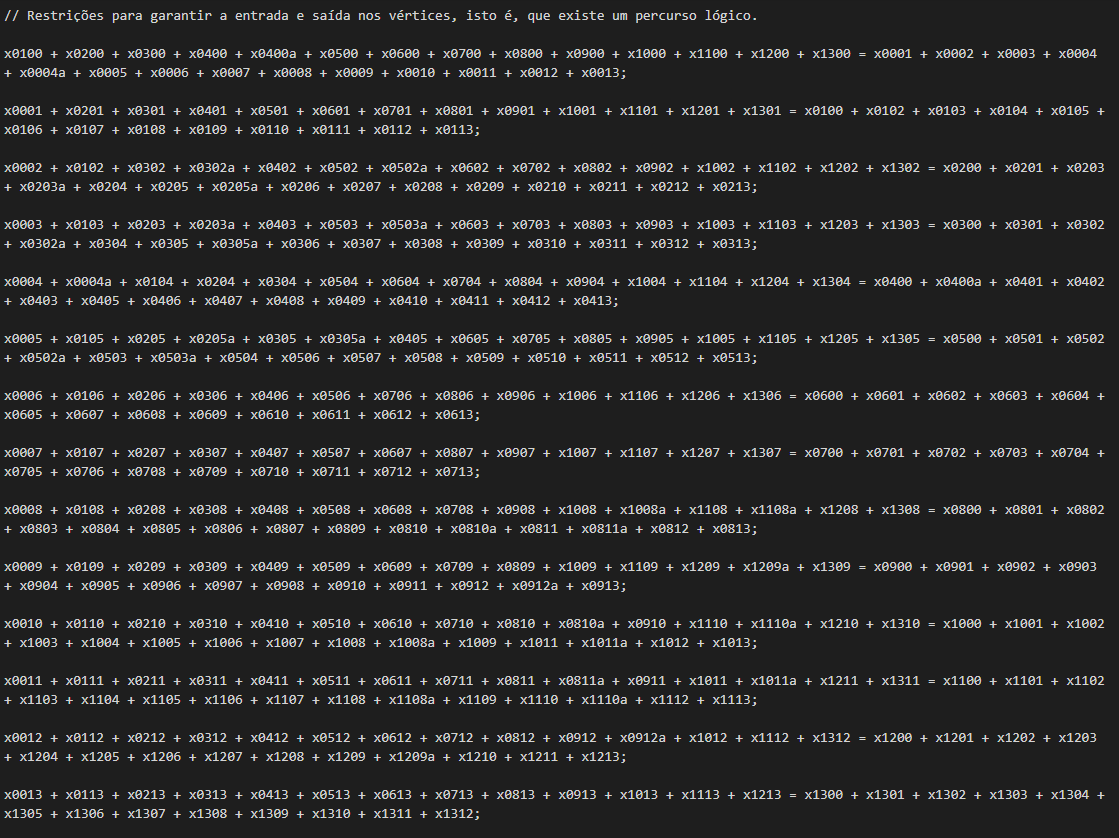
\includegraphics[width=1\textwidth]{images/main/restricoesEntradaSaida2.png}
\caption{Restrição para entrada e saída}
\end{figure}
\newpage
\subsection{Declaração de variáveis}

Declaração de variáveis no lpsolve como do tipo inteiro.

\begin{figure}[h!]
\centering
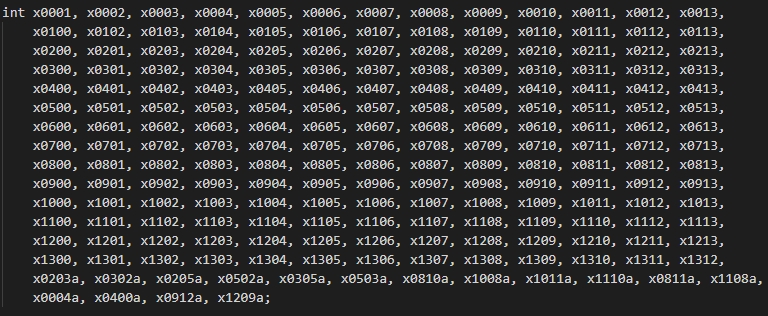
\includegraphics[width=1\textwidth]{images/main/declaracao.png}
\caption{Declaração de variáveis}
\end{figure}
\newpage

\section{Outputs}
Nas figuras seguintes encontram-se os diversos outputs obtidos pelo modelo.
\subsection{Output da solução}

Na figura abaixo encontra-se o output do modelo com possibilidades de percursos, tendo sido encontrado o percurso óptimo

\begin{figure}[h!]
\centering
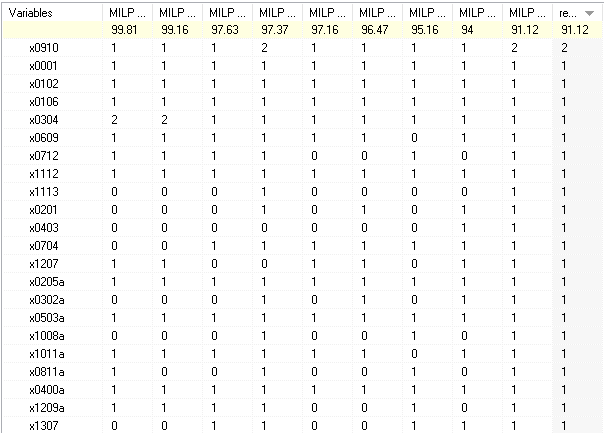
\includegraphics[width=.4\textwidth]{images/main/percursoOptimo.png}
\caption{Percurso ótimo}
\end{figure}

\subsection{Output Lpsolve}

\begin{figure}[h!]
\centering
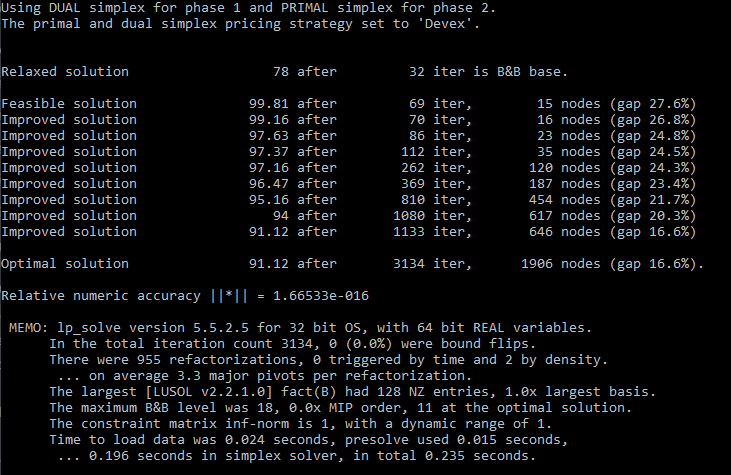
\includegraphics[width=.85\textwidth]{images/main/outputLPSolve.png}
\caption{Output produzido}
\end{figure}

\subsection{Exemplo de Percurso}

Como foi possível verificar anteriormente, o drone percorre todas as arestas necessárias, efetuando também um trajeto entre 11 e 13, onde não existe aresta. A distância total percorrida para este percurso, como indicada pelo lpsolve, é de 91.12.

Na figura seguinte encontra-se um exemplo de um percurso possível (as setas mudam de cor para melhorar a inspecção, de forma a tentar remover ambiguidade e mostrar mais claramente o percurso).


\begin{figure}[h!]
\centering
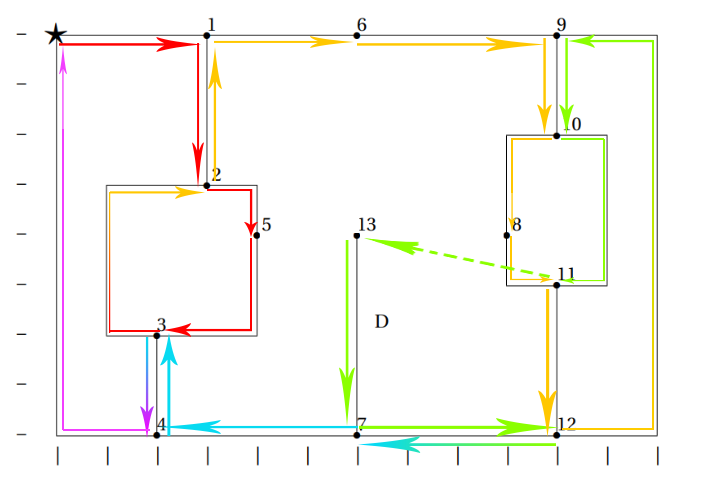
\includegraphics[width=.85\textwidth]{images/main/circuitofinal.png}
\caption{Exemplo circuito realizado}
\end{figure}

Desta forma validamos a solução óptima, mostrando que a solução proposta é admissível e correta, e vai ao encontro das necessidades propostas pelo enunciado, percorrendo todos os vértices e sendo um caminho válido.
